\documentclass{beamer}
\usepackage[utf8]{inputenc}

\usetheme{Madrid}
\usecolortheme{default}
\usepackage{amsmath,amssymb,amsfonts,amsthm}
\usepackage{txfonts}
\usepackage{tkz-euclide}
\usepackage{listings}
\usepackage{adjustbox}
\usepackage{array}
\usepackage{tabularx}
\usepackage{gvv}
\usepackage{lmodern}
\usepackage{circuitikz}
\usepackage{tikz}
\usepackage{graphicx}

\setbeamertemplate{page number in head/foot}[totalframenumber]

\usepackage{tcolorbox}
\tcbuselibrary{minted,breakable,xparse,skins}

\definecolor{bg}{gray}{0.95}
\DeclareTCBListing{mintedbox}{O{}m!O{}}{%
  breakable=true,
  listing engine=minted,
  listing only,
  minted language=#2,
  minted style=default,
  minted options={%
    linenos,
    gobble=0,
    breaklines=true,
    breakafter=,,
    fontsize=\small,
    numbersep=8pt,
    #1},
  boxsep=0pt,
  left skip=0pt,
  right skip=0pt,
  left=25pt,
  right=0pt,
  top=3pt,
  bottom=3pt,
  arc=5pt,
  leftrule=0pt,
  rightrule=0pt,
  bottomrule=2pt,
  toprule=2pt,
  colback=bg,
  colframe=orange!70,
  enhanced,
  overlay={%
    \begin{tcbclipinterior}
    \fill[orange!20!white] (frame.south west) rectangle ([xshift=20pt]frame.north west);
    \end{tcbclipinterior}},
  #3,
}


\lstset{
    language=C,
    basicstyle=\ttfamily\small,
    keywordstyle=\color{blue},
    stringstyle=\color{orange},
    commentstyle=\color{green!60!black},
    numbers=left,
    numberstyle=\tiny\color{gray},
    breaklines=true,
    showstringspaces=false,
}

\title{4.6.1}
\date{September 8, 2025}
\author{Bhargav - EE25BTECH11013}

\begin{document}

\frame{\titlepage}

\begin{frame}{Question}
The distance between the parallel planes
\begin{align}
2x + y - 2z - 6 = 0
\end{align}
\begin{align}
4x + 2y - 4z = 0
\end{align}
\end{frame}

\begin{frame}{Solution}
The $2$ given planes are parallel since their normal vectors are the same\\

The normal vector of the planes $\vec{n}$ is
\begin{align}
\vec{n} = \myvec{2 \\ 1 \\ -2}
\end{align}
\end{frame}

\begin{frame}{Solution}
The distance between the planes is given by this formula
\begin{align}
\text{Distance} = \frac{\abs{d_1 - d_2}}{\norm{\vec{n}}}
\end{align}

Where $d_1 = 6$ and $d_2 = 0$
\begin{align}
{\norm{\vec{n}}} = \brak{\sqrt{\brak{2}^2 + \brak{1}^2 + \brak{-2}^2}} = 3
\end{align}

\end{frame}

\begin{frame}{Solution}
Substituting these values in the Distance formula, we get\\
\begin{align}
\therefore \text{Distance} = \frac{\abs{6-0}}{3}
\end{align}

\begin{align}
\text{Distance} = 2
\end{align}
\end{frame}



\begin{frame}[fragile]
    \frametitle{C Code }

    \begin{lstlisting}


#include <math.h>
double norm(double *n) {
    return sqrt(n[0]*n[0] + n[1]*n[1] + n[2]*n[2]);
}
double plane_distance(double *n, double a, double b) {
    double num = fabs(a - b);
    double denom = norm(n);
    return num / denom;
}



    \end{lstlisting}
\end{frame}

\begin{frame}[fragile]
    \frametitle{Python + C Code }

    \begin{lstlisting}
import numpy as np
import matplotlib.pyplot as plt
import ctypes
lib = ctypes.CDLL('./libdistance.so')
lib.plane_distance.argtypes = [ctypes.POINTER(ctypes.c_double), ctypes.c_double, ctypes.c_double]
lib.plane_distance.restype = ctypes.c_double
n = np.array([2.0, 1.0, -2.0], dtype=np.double)
a = -6.0
b = 0.0
n_ptr = n.ctypes.data_as(ctypes.POINTER(ctypes.c_double))
dist = lib.plane_distance(n_ptr, a, b)
print('Distance =', dist)
fig = plt.figure()
ax3d = fig.add_subplot(projection='3d')
x, y = np.meshgrid(range(-10, 11), range(-10, 11))
z1 = (2*x + y - 6) / 2
z2 = (2*x + y) / 2

    \end{lstlisting}
\end{frame}

\begin{frame}[fragile]
    \frametitle{Python + C Code }

    \begin{lstlisting}
ax3d.plot_surface(x, y, z1, alpha=0.5, color='blue')
ax3d.plot_surface(x, y, z2, alpha=0.5, color='red')
ax3d.plot([], [], [], color='blue', label='2x + y - 2z - 6 = 0')
ax3d.plot([], [], [], color='red', label='2x + y - 2z = 0')
ax3d.set_xlabel('X')
ax3d.set_ylabel('Y')
ax3d.set_zlabel('Z')
ax3d.set_title(f'Two Parallel Planes\nDistance = {dist}')
ax3d.legend(loc='upper right')
plt.savefig('/Users/bhargavkrish/Desktop/BackupMatrix/ee25btech11013/matgeo/4.6.1/figs/Figure_1.png')
plt.show()

    \end{lstlisting}
\end{frame}

\begin{frame}[fragile]
    \frametitle{Python Code }

    \begin{lstlisting}
import numpy as np
import matplotlib.pyplot as plt
def distance(n, a, b):
    n = np.array(n, dtype=float)
    return abs(a - b) / np.linalg.norm(n)
n = np.array([2, 1, -2])
a = -6
b = 0
dist = distance(n, a, b)
print('Distance =', dist)
fig = plt.figure()
ax3d = fig.add_subplot(projection='3d')
x, y = np.meshgrid(range(-10, 11), range(-10, 11))
z1 = (2*x + y - 6) / 2
z2 = (2*x + y) / 2
ax3d.plot_surface(x, y, z1, alpha=0.5, color='blue')
ax3d.plot_surface(x, y, z2, alpha=0.5, color='red')


    \end{lstlisting}
\end{frame}

\begin{frame}[fragile]
    \frametitle{Python Code }

    \begin{lstlisting}

ax3d.plot([], [], [], color='blue', label='2x + y - 2z - 6 = 0')
ax3d.plot([], [], [], color='red', label='2x + y - 2z = 0')
ax3d.set_xlabel('X')
ax3d.set_ylabel('Y')
ax3d.set_zlabel('Z')
ax3d.set_title(f'Two Parallel Planes\nDistance = {dist}')
ax3d.legend(loc='upper right')
plt.savefig('/Users/bhargavkrish/Desktop/BackupMatrix/ee25btech11013/matgeo/4.6.1/figs/Figure_1.png')
plt.show()



    \end{lstlisting}
\end{frame}



\begin{frame}{Figure}
\begin{figure}[h!]
    \centering
    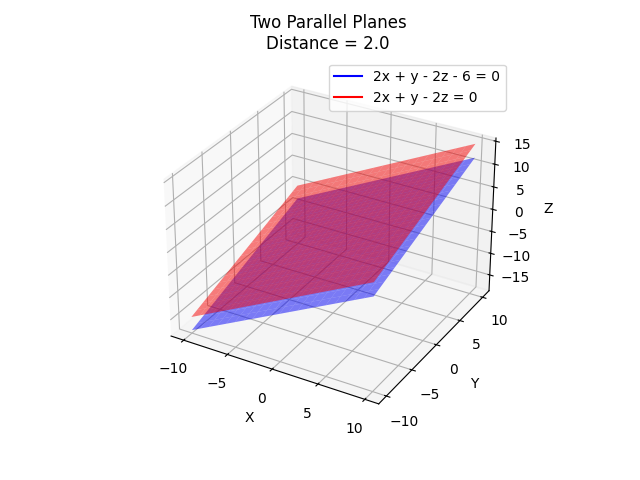
\includegraphics[height=0.5\textheight, keepaspectratio]{figs/Figure_1.png}
\end{figure}
\end{frame}

\end{document}
